\newpage
\subsection{Лабораторная работа №5. Функции и процедуры}
Задачи к лабораторной работе №5:
\begin{enumerate}
    \item Написать функцию, формирующую ФИО из фамилии, имени и отчества в формате «Фамилия И. О.».
    \item Написать процедуру, которая принимает атрибуты нескольких связанных сущностей, находит существующие записи или добавляет новые, а затем изменяет данные, отображаемые в представлении.
\end{enumerate}

\subsubsection{Создание функции}
В таблицах \texttt{student} и \texttt{employee} фамилия, имя и отчество хранятся в отдельных полях. Для формирования краткой записи ФИО создана функция \texttt{format\_full\_name}. Функция принимает три значения, удаляет пробелы по краям и добавляет к первым буквам имени и отчества точки. Если отчество не задано, функция возвращает только фамилию и инициал имени.

Код функции и запрос для вывода трех исходных атрибутов вместе с результатом приведены в листинге~\ref{lst:lab5-name}.

\begin{lstlisting}[language=SQL, caption={Функция форматирования ФИО и запрос к ней}, label={lst:lab5-name}]
CREATE OR REPLACE FUNCTION format_full_name(
    p_last_name TEXT,
    p_first_name TEXT,
    p_middle_name TEXT
)
RETURNS TEXT
LANGUAGE SQL
IMMUTABLE
AS $$
    SELECT concat_ws(
        ' ',
        NULLIF(btrim(p_last_name), ''),
        CASE
            WHEN NULLIF(btrim(p_first_name), '') IS NOT NULL
            THEN upper(left(btrim(p_first_name), 1)) ||
                 CASE
                     WHEN NULLIF(btrim(p_middle_name), '') IS NOT NULL THEN '.'
                     ELSE ''
                 END
        END,
        CASE
            WHEN NULLIF(btrim(p_middle_name), '') IS NOT NULL
            THEN upper(left(btrim(p_middle_name), 1)) || '.'
        END
    );
$$;

SELECT
    last_name,
    first_name,
    middle_name,
    format_full_name(last_name, first_name, middle_name) AS formatted_name
FROM student
ORDER BY student_id
LIMIT 15;

SELECT format_full_name('Predovic', 'Anastasia', NULL) AS name_without_middle;
\end{lstlisting}

В таблице \texttt{student} ФИО сформированы из английских имён и фамилий библиотеки \texttt{gofakeit}. Например, для студента \texttt{Predovic Anastasia Christiana} функция возвращает \texttt{Predovic A. C.}. Если отчество не задано, результатом будет \texttt{Predovic A} без точки в конце. Фактический вывод для 15 студентов и проверка варианта без отчества представлены на рисунке~\ref{fig:lab5-name-result}.

\begin{figure}[H]
    \centering
    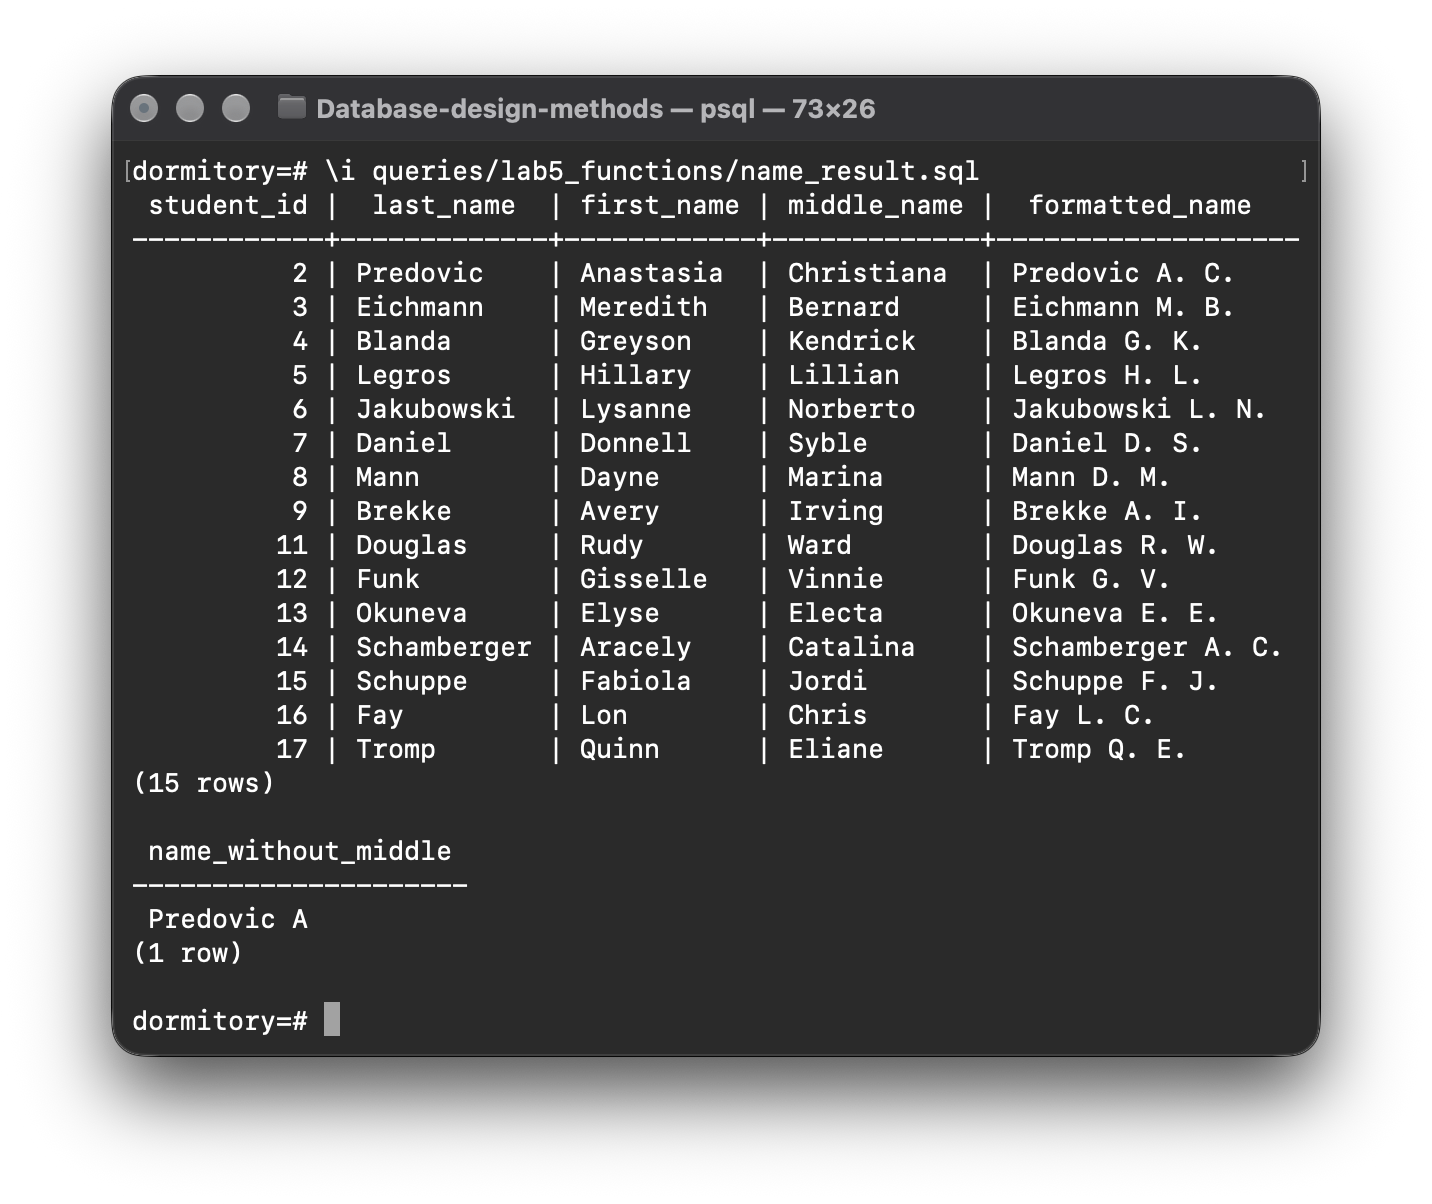
\includegraphics[width=0.9\textwidth]{figures/lab5_user_name_result.png}
    \caption{Результат форматирования ФИО студентов из базы данных}
    \label{fig:lab5-name-result}
\end{figure}

\subsubsection{Блок-схема процедуры}
Для предметной области общежития процедура регистрирует заселение студента и связанный с ним платёж. Помимо данных студента передаются сведения о сотруднике, здании, типе комнаты, этаже, датах, способе оплаты и сумме. Перед добавлением записей процедура проверяет наличие каждой сущности по переданным атрибутам. Блок-схема алгоритма приведена на рисунке~\ref{fig:lab5-procedure}.

\begin{figure}[H]
    \centering
    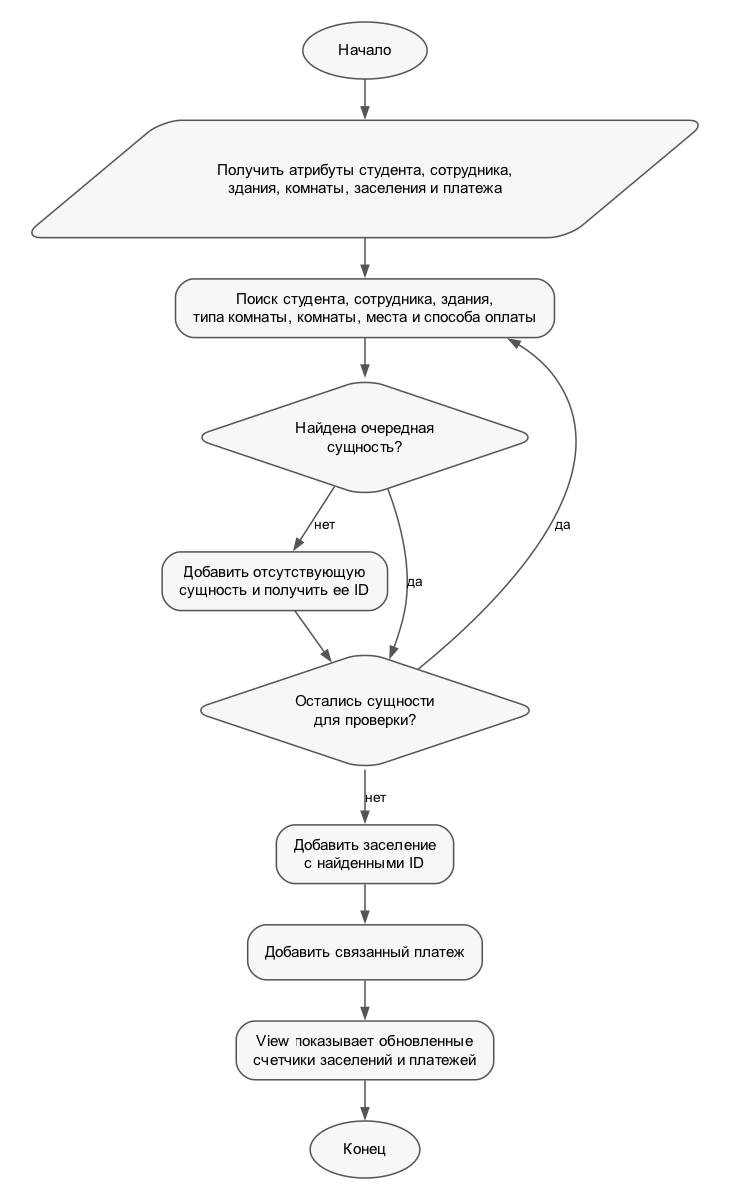
\includegraphics[width=0.72\textwidth]{figures/lab5_procedure.png}
    \caption{Блок-схема процедуры регистрации заселения}
    \label{fig:lab5-procedure}
\end{figure}

\subsubsection{Процедура регистрации заселения}
Процедура \texttt{register\_settlement} принимает 17 параметров. Сначала она ищет студента и сотрудника по полному набору переданных полей. Затем аналогично проверяет здание, тип комнаты, комнату, место и способ оплаты. Для найденных сущностей используются их идентификаторы; отсутствующие записи добавляются. После этого создаются новое заселение и платёж.

Так как сводная таблица \texttt{student\_settlement\_payment\_counts} в лабораторной работе №2 была заменена таблицей с триггерами, процедура также создаёт начальную строку счётчиков для нового студента. Триггеры заселения и платежа увеличивают соответствующие значения.

Код процедуры приведён в листинге~\ref{lst:lab5-procedure}.

\begin{lstlisting}[language=SQL, caption={Процедура регистрации заселения}, label={lst:lab5-procedure}]
CREATE OR REPLACE PROCEDURE register_settlement(
    p_student_last_name TEXT,
    p_student_first_name TEXT,
    p_student_middle_name TEXT,
    p_student_passport_data TEXT,
    p_employee_last_name TEXT,
    p_employee_first_name TEXT,
    p_employee_middle_name TEXT,
    p_employee_passport_data TEXT,
    p_employee_position TEXT,
    p_building_address TEXT,
    p_room_type_name TEXT,
    p_place_level INTEGER,
    p_move_in_date DATE,
    p_move_out_date DATE,
    p_payment_method_name TEXT,
    p_payment_amount NUMERIC(10, 2),
    p_payment_date DATE
)
LANGUAGE plpgsql
AS $$
DECLARE
    v_student_id INTEGER;
    v_employee_id INTEGER;
    v_building_id INTEGER;
    v_room_type_id INTEGER;
    v_room_id INTEGER;
    v_place_id INTEGER;
    v_payment_method_id INTEGER;
    v_settlement_id INTEGER;
BEGIN
    SELECT student_id INTO v_student_id FROM student
    WHERE last_name IS NOT DISTINCT FROM p_student_last_name
      AND first_name IS NOT DISTINCT FROM p_student_first_name
      AND middle_name IS NOT DISTINCT FROM p_student_middle_name
      AND passport_data IS NOT DISTINCT FROM p_student_passport_data
    ORDER BY student_id LIMIT 1;
    IF v_student_id IS NULL THEN
        INSERT INTO student (last_name, first_name, middle_name, passport_data)
        VALUES (p_student_last_name, p_student_first_name, p_student_middle_name, p_student_passport_data)
        RETURNING student_id INTO v_student_id;
    END IF;

    INSERT INTO student_settlement_payment_counts
        (student_id, last_name, first_name, middle_name, settlement_count, payment_count)
    SELECT v_student_id, p_student_last_name, p_student_first_name,
           p_student_middle_name, 0, 0
    ON CONFLICT (student_id) DO NOTHING;

    SELECT employee_id INTO v_employee_id FROM employee
    WHERE last_name IS NOT DISTINCT FROM p_employee_last_name
      AND first_name IS NOT DISTINCT FROM p_employee_first_name
      AND middle_name IS NOT DISTINCT FROM p_employee_middle_name
      AND passport_data IS NOT DISTINCT FROM p_employee_passport_data
      AND position IS NOT DISTINCT FROM p_employee_position
    ORDER BY employee_id LIMIT 1;
    IF v_employee_id IS NULL THEN
        INSERT INTO employee (last_name, first_name, middle_name, passport_data, position)
        VALUES (p_employee_last_name, p_employee_first_name, p_employee_middle_name,
                p_employee_passport_data, p_employee_position)
        RETURNING employee_id INTO v_employee_id;
    END IF;

    SELECT building_id INTO v_building_id FROM building
    WHERE building_address IS NOT DISTINCT FROM p_building_address
    ORDER BY building_id LIMIT 1;
    IF v_building_id IS NULL THEN
        INSERT INTO building (building_address) VALUES (p_building_address)
        RETURNING building_id INTO v_building_id;
    END IF;

    SELECT room_type_id INTO v_room_type_id FROM room_type
    WHERE type_name IS NOT DISTINCT FROM p_room_type_name
    ORDER BY room_type_id LIMIT 1;
    IF v_room_type_id IS NULL THEN
        INSERT INTO room_type (type_name) VALUES (p_room_type_name)
        RETURNING room_type_id INTO v_room_type_id;
    END IF;

    SELECT room_id INTO v_room_id FROM room
    WHERE building_id = v_building_id AND room_type_id = v_room_type_id
    ORDER BY room_id LIMIT 1;
    IF v_room_id IS NULL THEN
        INSERT INTO room (building_id, room_type_id)
        VALUES (v_building_id, v_room_type_id)
        RETURNING room_id INTO v_room_id;
    END IF;

    SELECT place_id INTO v_place_id FROM place
    WHERE room_id = v_room_id AND level = p_place_level
    ORDER BY place_id LIMIT 1;
    IF v_place_id IS NULL THEN
        INSERT INTO place (room_id, level) VALUES (v_room_id, p_place_level)
        RETURNING place_id INTO v_place_id;
    END IF;

    SELECT payment_method_id INTO v_payment_method_id FROM payment_method
    WHERE method_name IS NOT DISTINCT FROM p_payment_method_name
    ORDER BY payment_method_id LIMIT 1;
    IF v_payment_method_id IS NULL THEN
        INSERT INTO payment_method (method_name) VALUES (p_payment_method_name)
        RETURNING payment_method_id INTO v_payment_method_id;
    END IF;

    INSERT INTO settlement (student_id, employee_id, place_id, move_in_date, move_out_date)
    VALUES (v_student_id, v_employee_id, v_place_id, p_move_in_date, p_move_out_date)
    RETURNING settlement_id INTO v_settlement_id;
    INSERT INTO payment (settlement_id, payment_method_id, payment_amount, payment_date)
    VALUES (v_settlement_id, v_payment_method_id, p_payment_amount, p_payment_date);
END;
$$;

\end{lstlisting}

Создание функции и процедуры в базе данных подтверждается результатом команд \texttt{CREATE FUNCTION} и \texttt{CREATE PROCEDURE}, представленным на рисунке~\ref{fig:lab5-create-result}.

\begin{figure}[H]
    \centering
    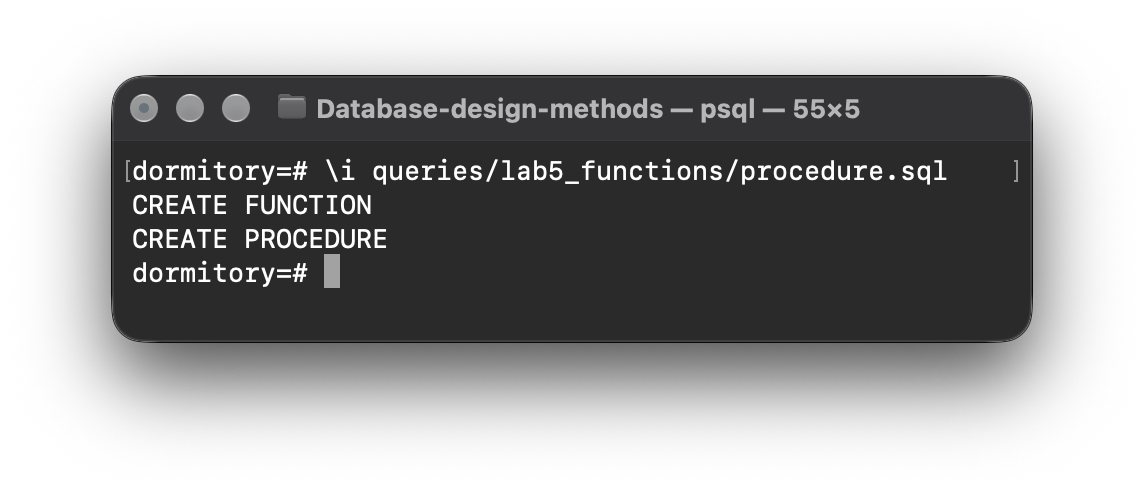
\includegraphics[width=0.75\textwidth]{figures/lab5_user_procedure_created.png}
    \caption{Создание функции и процедуры в базе данных}
    \label{fig:lab5-create-result}
\end{figure}

Проверка процедуры выполнена для трёх способов использования:
\begin{enumerate}
    \item все сущности отсутствуют и создаются процедурой;
    \item все сущности уже существуют, процедура использует найденные идентификаторы;
    \item студент отсутствует, а сотрудник, здание, тип комнаты, комната, место и способ оплаты уже существуют.
\end{enumerate}

Сценарии вызова приведены в листинге~\ref{lst:lab5-scenarios}. Фактический вывод терминала по всем трём сценариям представлен на рисунке~\ref{fig:lab5-proc-results}.

\begin{lstlisting}[language=SQL, caption={Вызовы процедуры для разных сценариев}, label={lst:lab5-scenarios}]
-- Новый студент и новые связанные сущности
CALL register_settlement(
    'Predovic', 'Anastasia', 'Christiana', '9999999999',
    'Lind', 'Nolan', 'Simone', '9999999998', 'Agent',
    '500 Codex Way, Sampleton, Maine 00001', 'suite', 2,
    DATE '2025-09-01', NULL, 'card', 1500.00, DATE '2025-09-01'
);

-- Все сущности найдены в базе данных
CALL register_settlement(
    'Predovic', 'Anastasia', 'Christiana', '4618268510',
    'Lind', 'Nolan', 'Simone', '2506250516', 'Agent',
    '38713 East Cliffsberg, Durham, Delaware 25965', 'квартирный', 3,
    DATE '2025-09-01', NULL, 'карта', 1500.00, DATE '2025-09-01'
);

-- Новый студент при существующих справочных сущностях
CALL register_settlement(
    'Predovic', 'Anastasia', 'Christiana', '9999999997',
    'Lind', 'Nolan', 'Simone', '2506250516', 'Agent',
    '38713 East Cliffsberg, Durham, Delaware 25965', 'квартирный', 3,
    DATE '2025-09-01', NULL, 'карта', 1500.00, DATE '2025-09-01'
);
\end{lstlisting}

В первом сценарии создан студент с идентификатором 5007; в сводной таблице для него указаны одно заселение и один платёж. Во втором сценарии использован уже существующий студент с идентификатором 2: значения счётчиков изменились с 6 и 80 до 7 и 81. В третьем сценарии создан новый студент с идентификатором 5008 при повторном использовании существующих справочных сущностей; оба счётчика равны единице.

\begin{figure}[H]
    \centering
    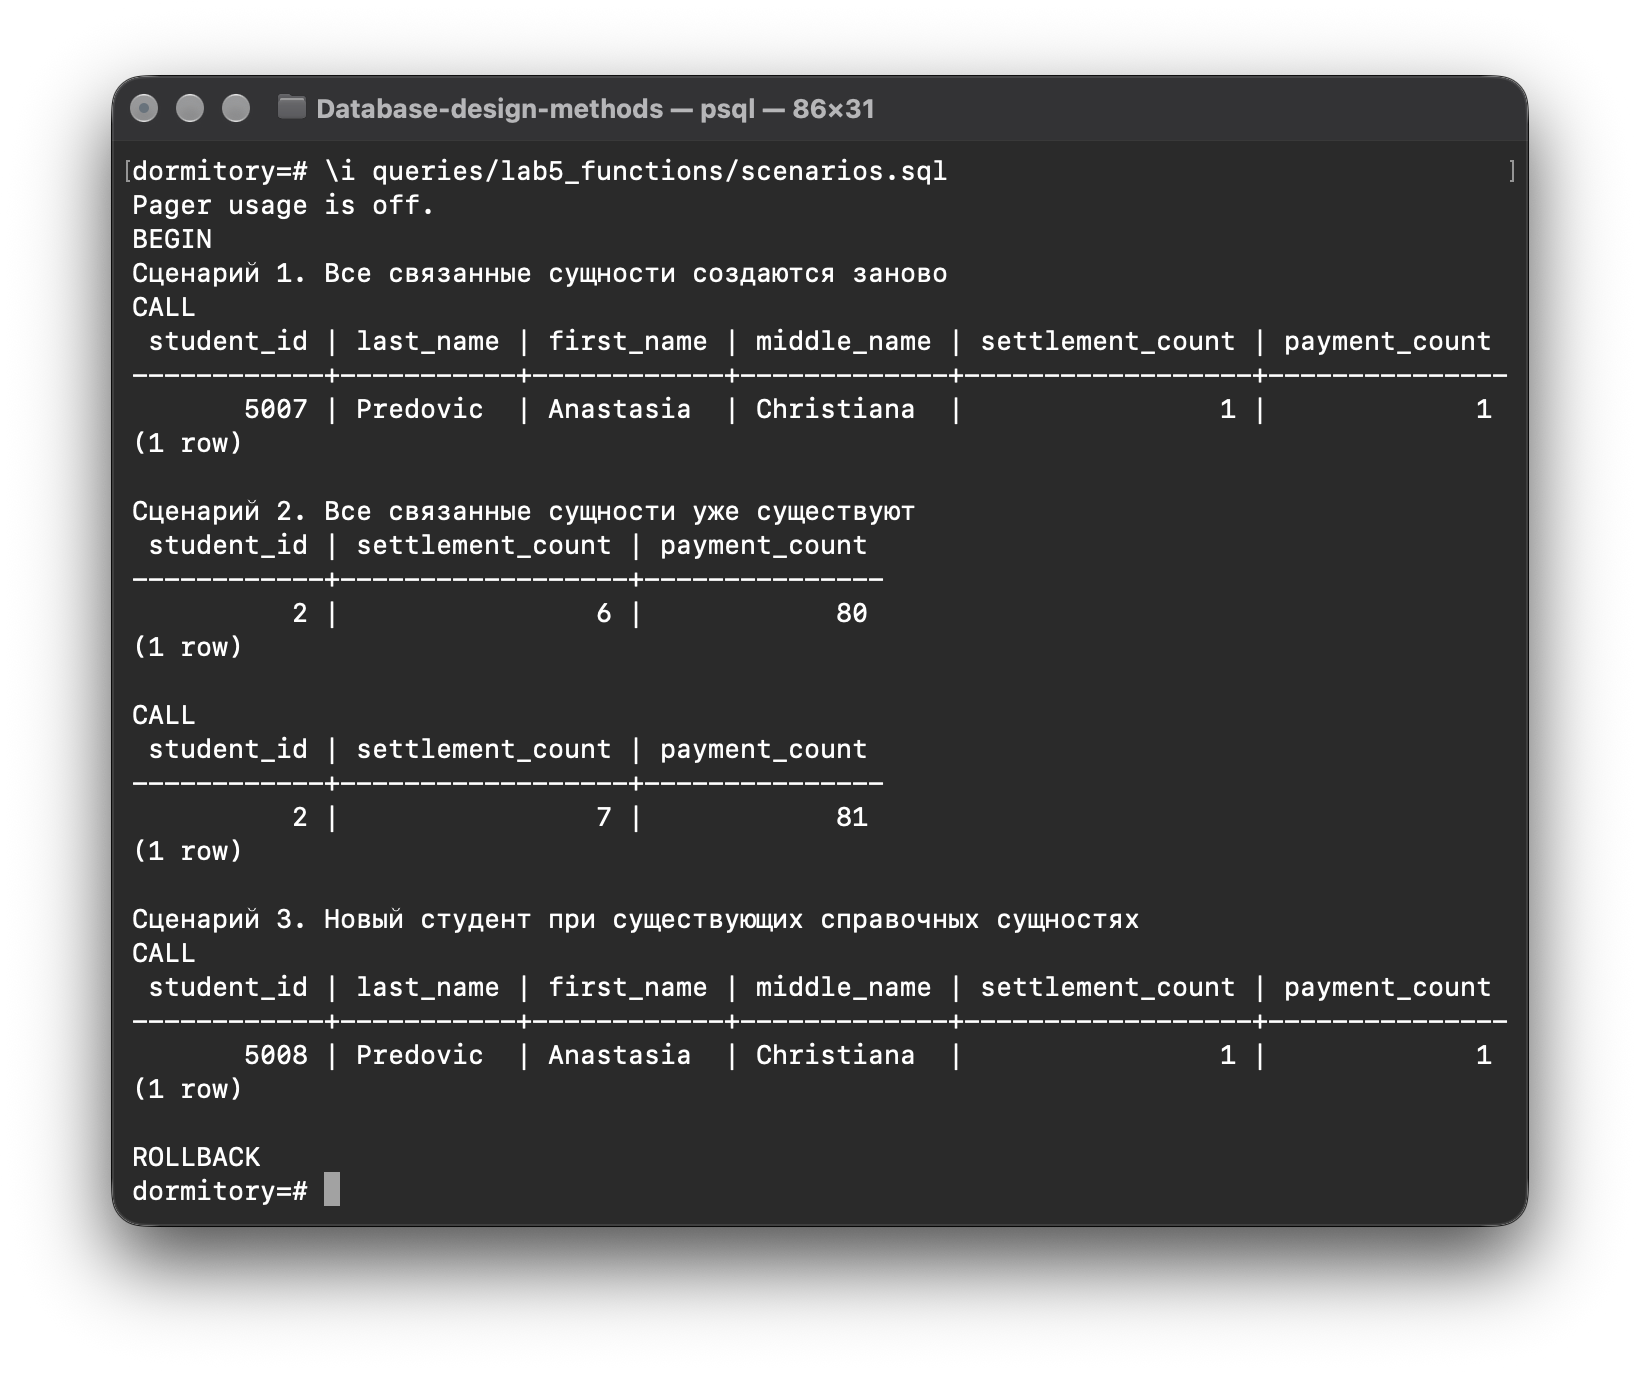
\includegraphics[width=0.92\textwidth]{figures/lab5_user_scenarios.png}
    \caption{Результаты работы процедуры в трёх сценариях}
    \label{fig:lab5-proc-results}
\end{figure}

Вызовы выполнялись внутри транзакции; в конце сценария выполнен \texttt{ROLLBACK}, поэтому тестовые строки отменены, а сводная таблица осталась без новых записей. Значения последовательностей \texttt{SERIAL} в PostgreSQL не откатываются, поэтому следующие автоматически назначаемые идентификаторы будут больше показанных на снимках. Сводная таблица отобразила результаты до отмены транзакции.

Для проверки результата процедуры выполняется запрос:

\begin{lstlisting}[language=SQL, caption={Проверка изменения представления}, label={lst:lab5-view-check}]
SELECT
    student_id,
    last_name,
    first_name,
    middle_name,
    settlement_count,
    payment_count
FROM student_settlement_payment_counts
WHERE last_name = 'Predovic' AND first_name = 'Anastasia'
ORDER BY student_id;
\end{lstlisting}

Для нового студента оба счётчика в сводной таблице после добавления одной записи будут равны единице. При существующем студенте процедура увеличивает его счётчики с помощью триггеров, а повторные справочные записи не добавляются.
